\subsection{Spark}
Apache Spark is a general purpose cluster-computing system, that offers a high level programming language API as well as a set of high-level tools, for SQL data, machine learning and graph processing. ~\cite{sparkintro} 

A Spark application is a user-application that is run by the “Driver Program”, see figure \ref{fig:spark}, in which a “Spark Context” object is defined. The Spark Context can connect to several cluster managers; Spark Standalone, Yarn, Mesos, etc. For the work in this article, the default standalone manager is used. When connected, the Spark Context gather “Executors”, which are running processes on the worker nodes. We naturally want worker nodes to also be Hadoop data nodes, as to not limit the computation from slow network transfer speeds. Each driver program gets it’s own set of executors which isolates the programs from each others. If programs need to share data, this has to be done through an external storage system like HDFS.

By default the standalone cluster manager handle worker node failure, but as the manager uses a single-node master for work scheduling, the manager has a single-point of failure by default. External services such as Apache ZooKeeper can be used to address this problem, by distributing and coordination the scheduling. The cluster for this work is set up much like HDFS. One node acts as a central node, running the driver program and cluster manager, the remaining 3 nodes are worker nodes. The worker nodes and data nodes are set up on the same machines, as to avoid unnecessary load on the network.~\cite{sparkcluster} - The cluster manager interfaces with Hadoop and assign work to be done as close to the data as possible. In the general case, this means that the executors will only access data from the worker nodes own disk??-no source for last statement.

\begin{figure}	
	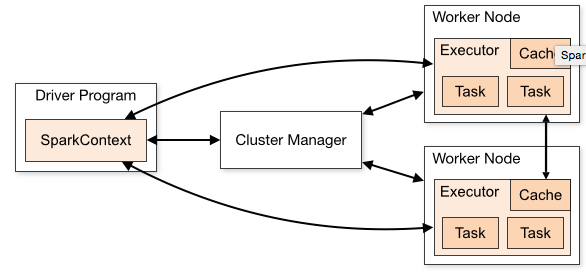
\includegraphics[width=\textwidth]{cluster/images/sparkoverview.png} 
	\label{fig:spark} 
\end{figure}
